% ============================================================
%  Thesis Defense — 20 slides / 20 minutes
%  Leakage-Aware Brain Tumor Classification with StyleGAN2-ADA
%  Junwei He Mai
% ============================================================
\documentclass[aspectratio=169]{beamer}

\usetheme{Madrid}
\usecolortheme{whale}
\useoutertheme[subsection=false]{miniframes}
\usefonttheme{professionalfonts}
\setbeamertemplate{navigation symbols}{}
\setbeamertemplate{caption}[numbered]

% ── Fix miniframes colors: dark navy bg, white text & dots ──
\setbeamercolor{section in head/foot}{fg=white, bg=structure.fg!20!black}
\setbeamercolor{section in head/foot shaded}{fg=white!45!black, bg=structure.fg!20!black}
\setbeamercolor{mini frame}{fg=white, bg=white}
\setbeamertemplate{mini frame}[box]

\usepackage[utf8]{inputenc}
\usepackage[T1]{fontenc}
\usepackage{lmodern}
\usepackage{booktabs}
\usepackage{multirow}
\usepackage{amsmath}
\usepackage{xcolor}
\usepackage{tikz}
\usetikzlibrary{arrows.meta, positioning, fit, shapes.geometric, backgrounds, calc}
\usepackage{animate}
\usepackage{pgfplots}
\pgfplotsset{compat=1.18}
\usepackage{grffile}

\definecolor{myblue}{RGB}{0,84,166}
\definecolor{mygreen}{RGB}{0,150,80}
\definecolor{myred}{RGB}{200,30,30}
\definecolor{mygold}{RGB}{180,130,0}
\definecolor{mypurple}{RGB}{120,55,160}

% ============================================================
%  SLIDE 1 — TITLE
% ============================================================
\title[Brain Tumor · StyleGAN-C]{%
  Explainable Brain Tumor Classification\\
  via Generation Using Conditional StyleGANs and CNNs}

\author[Junwei He Mai]{
  \textbf{Author:} Junwei He Mai\\[6pt]
  \small
  \textbf{Advisor:} Juan Vel\'asquez Silva \quad
  \textbf{Co-advisor:} Yong Zhang\\[6pt]
  \textbf{Committee:}\\[2pt]
  Ingeborg L\'opez Liberona \enspace·\enspace Denis Saur\'e Valenzuela
}
\institute[]{%
  \footnotesize
  Thesis for \textbf{Master of Data Science} and \textbf{Industrial Engineering}\\[2pt]
  Universidad de Chile%
}
\date{May 8, 2026}

\newcommand{\uchilelogo}{D:/tesis/thesis-brain-tumor-stylegan2/latex/img/departamentos/uchile}

\newcommand{\customtitlepage}{%
\begin{frame}
  \titlepage
\end{frame}
}

\begin{document}

\customtitlepage

% ============================================================
%  SLIDE 2 — AGENDA
% ============================================================
\begin{frame}{Agenda}
  \footnotesize
  \tableofcontents
\end{frame}

% ============================================================
%  SLIDE 3 — CONTEXT
% ============================================================
\section{Context}
\begin{frame}{Context}
  \begin{columns}
    \begin{column}{0.55\textwidth}
      \textbf{Brain tumors}
      \begin{itemize}
        \item Represent a major health issue due to high mortality rate
        \item Diagnosed via various imaging modalities (MRI, CT, PET)
        \item Three main types:\\[3pt]
          \quad \textcolor{myblue}{\textbf{Glioma}}: intra-axial, malignant\\
          \quad \textcolor{mygreen}{\textbf{Meningioma}}: extra-axial, slow-growing\\
          \quad \textcolor{mygold}{\textbf{Pituitary}}: sellar, benign
        \item \textbf{Data scarcity:} few public datasets
              with reliable patient-level annotation
        \item \textbf{Low clinical adoption:} clinicians do not trust black-box models
      \end{itemize}
      \vspace{0.3em}
      \textbf{Role of AI:} provide diagnostic support and
      clinically interpretable classification
    \end{column}
    \begin{column}{0.42\textwidth}
      \begin{block}{Dataset}
        \textbf{Figshare Brain Tumor MRI}\\
        (Cheng et al., 2015) · resized to $256\times256$\\[6pt]
        \begin{tabular}{lcc}
          \toprule
          Class & Patients & Slices \\
          \midrule
          \textcolor{myblue}{Glioma}      & 89 & 1{,}426 \\
          \textcolor{mygreen}{Meningioma}  & 82 & \phantom{0}708 \\
          \textcolor{mygold}{Pituitary}   & 62 & \phantom{0}930 \\
          \midrule
          \textbf{Total} & \textbf{233} & \textbf{3{,}064} \\
          \bottomrule
        \end{tabular}
        \vspace{4pt}
        {\scriptsize \textcolor{myred}{\textbf{Imbalance:}}
        $\sim$2:1 glioma vs.\ meningioma}
      \end{block}
    \end{column}
  \end{columns}
\end{frame}

% ============================================================
%  SLIDE 3 — PROBLEM
% ============================================================
\section{Problem}
\begin{frame}{The Problem: Why Is This Hard?}
  \footnotesize
  {\setbeamercolor{block title alerted}{bg=myred!85, fg=white}%
   \setbeamercolor{block body alerted}{bg=myred!10, fg=black}%
  \begin{alertblock}{P1 · Lack of Explainability}
    Black-box models. Clinicians cannot trust a prediction without an explanation.\\[1pt]
    \textcolor{mygreen}{\textit{Consequence: no explanation $\Rightarrow$ no clinical adoption.}}
  \end{alertblock}}
  \vspace{-0.4em}
  {\setbeamercolor{block title alerted}{bg=mygold!85, fg=white}%
   \setbeamercolor{block body alerted}{bg=mygold!10, fg=black}%
  \begin{alertblock}{P2 · Scarcity of Data}
    Few public MRI datasets are available with reliable patient-level annotation.\\[1pt]
    \textcolor{mygreen}{\textit{Consequence: no data $\Rightarrow$ no good model.}}
  \end{alertblock}}
  \vspace{-0.4em}
  {\setbeamercolor{block title alerted}{bg=mypurple!85, fg=white}%
   \setbeamercolor{block body alerted}{bg=mypurple!10, fg=black}%
  \begin{alertblock}{P3 · Data Leakage}
    No SOTA methodology enforces patient-level separation, so reported metrics are inflated.\\[1pt]
    \textcolor{mygreen}{\textit{Consequence: no clean evaluation $\Rightarrow$ no trustworthy metrics.}}
  \end{alertblock}}
\end{frame}

% ============================================================
%  SLIDE 4 — RESEARCH QUESTIONS & HYPOTHESES
% ============================================================
\section{Questions}
\begin{frame}{Research Questions}
  \footnotesize
  {\setbeamercolor{block title}{bg=myblue!85, fg=white}%
   \setbeamercolor{block body}{bg=myblue!10, fg=black}%
  \begin{block}{RQ1 · Generative validity}
    Do class-conditional MRI images generated by StyleGAN-C
    reach clinically acceptable levels of realism and diagnostic utility,
    as determined by neuroradiologist HITL ratings using
    structured Likert-style forms?
  \end{block}}
  \vspace{-0.4em}
  {\setbeamercolor{block title}{bg=mygreen!75, fg=white}%
   \setbeamercolor{block body}{bg=mygreen!10, fg=black}%
  \begin{block}{RQ2 · Classification impact}
    How does incorporating StyleGAN-C affect brain tumor MRI classification
    when used through (i) inference-by-generation via latent inversion and
    perceptual similarity, and (ii) synthetic data augmentation for CNN training?
  \end{block}}
  \vspace{-0.4em}
  {\setbeamercolor{block title}{bg=mygold!85, fg=white}%
   \setbeamercolor{block body}{bg=mygold!10, fg=black}%
  \begin{block}{RQ3 · Image-based explainability}
    Can image-based explainability methods that incorporate generative evidence
    provide clinically interpretable visual support that assists
    neuroradiologists in the diagnostic process?
  \end{block}}
\end{frame}

\begin{frame}{Hypotheses}
  \scriptsize
  {\setbeamercolor{block title example}{bg=myblue!85, fg=white}%
   \setbeamercolor{block body example}{bg=myblue!10, fg=black}%
  \begin{exampleblock}{$H_1$ · Generative validity}
    StyleGAN-C generates class-conditional brain tumor MRI slices that preserve
    relevant tumor-related anatomical structures, as reflected by high
    neuroradiologist HITL ratings.
  \end{exampleblock}}
  \vspace{-0.4em}
  {\setbeamercolor{block title example}{bg=mygreen!75, fg=white}%
   \setbeamercolor{block body example}{bg=mygreen!10, fg=black}%
  \begin{exampleblock}{$H_{2A}$ · Inversion-based classification}
    Optimization or encoder-based latent inversion in the StyleGAN-C latent space
    enables tumor classification with accuracy above 0.8.
  \end{exampleblock}}
  \vspace{-0.4em}
  {\setbeamercolor{block title example}{bg=mypurple!85, fg=white}%
   \setbeamercolor{block body example}{bg=mypurple!10, fg=black}%
  \begin{exampleblock}{$H_{2B}$ · GAN augmentation}
    Incorporating StyleGAN-C synthetic images into CNN training improves the
    confidence of its probabilistic predictions compared to real-only training.
  \end{exampleblock}}
  \vspace{-0.4em}
  {\setbeamercolor{block title example}{bg=mygold!85, fg=white}%
   \setbeamercolor{block body example}{bg=mygold!10, fg=black}%
  \begin{exampleblock}{$H_3$ · Explainability}
    Image-based XAI provides neuroradiologists more clinically useful and
    trustworthy support for brain tumor classification than no XAI.
  \end{exampleblock}}
\end{frame}

% ============================================================
%  SLIDES 5–7 — RELATED WORK
% ============================================================
\section{Related Work}
\begin{frame}{Related Work (1/4): GANs for Medical Image Synthesis}
  \begin{itemize}
    \item \textbf{DCGAN} (Ghassemi et al., 2020). \textbf{Creates} MRI slices from
          random noise. \emph{$64\times64$ · Figshare}
    \item \textbf{TumorGAN} (Li et al., 2020). \textbf{Transforms} healthy slices
          into tumor ones (pix2pix). \emph{$256\times256$ · BraTS 2017}
    \item \textbf{LR-cGAN} (Zhan et al., 2021). \textbf{Combines} MRI
          modalities (T1+T2 $\rightarrow$ FLAIR). \emph{$256\times256$ · BraTS 2015}
    \item \textbf{MCFDiffusion} (Zuo et al., 2025). \textbf{Combines} healthy and
          tumor regions via diffusion. \emph{$256\times256$ · LGG}
  \end{itemize}
  \vspace{0.3em}
  \begin{alertblock}{Gap}
    No prior generative model produces \textbf{class-conditional}
    brain tumor MRI at $256\times256$ across glioma, meningioma, and pituitary.
  \end{alertblock}
\end{frame}

\begin{frame}{Related Work (2/4): Classification on Figshare}
  \begin{itemize}
    \item \textbf{GLCM-SVM} (Cheng et al., 2015). \textbf{Extracts} handcrafted
          features (ROI partition + GLCM) and classifies with SVM.
          \emph{$512\times512$ · patient split · 92.3\% acc.}
    \item \textbf{Custom CNN} (Abiwinanda et al., 2018). \textbf{Trains} a small
          custom CNN at low resolution.
          \emph{$64\times64$ · split not reported · 94.7\% acc.}
    \item \textbf{GoogLeNet-TL} (Deepak et al., 2019). \textbf{Transfers} a
          pretrained GoogLeNet, then swaps softmax for a KNN/SVM classifier on
          the CNN features.
          \emph{$224\times224$ · patient split · 92.3\% (softmax) / 98.0\% (KNN)}
    \item \textbf{VGG16-SVM} (Rehman et al., 2019). \textbf{Benchmarks} AlexNet,
          GoogLeNet and VGG variants.
          \emph{$224\times224$ · split not reported · 94.6\% acc.}
  \end{itemize}
  \vspace{0.3em}
  \begin{alertblock}{Gap}
    Two of four works do not enforce patient-level separation,
    so reported metrics may be inflated.
  \end{alertblock}
\end{frame}

\begin{frame}{Related Work (3/4): Explainability}
  \begin{itemize}
    \item \textbf{Grad-CAM CNN} (Windisch et al., 2020). \textbf{Visualizes}
          class activations on a basic CNN for brain tumor detection.
          \emph{Multiclass brain MRI · Grad-CAM}
    \item \textbf{DenseNet + Grad-CAM} (Esmaeili et al., 2021). \textbf{Localizes}
          tumor regions and proposes a human-machine interaction loop.
          \emph{Multiclass brain MRI · Grad-CAM}
  \end{itemize}
  \vspace{0.3em}
  \begin{alertblock}{Gap}
    Prior XAI work is purely \textbf{post-hoc and qualitative}.
    None integrate HITL clinician ratings.
  \end{alertblock}
\end{frame}

\begin{frame}{Related Work (4/4): Comparative Table}
  \begin{center}
  \fontsize{7pt}{8pt}\selectfont
  \begin{tabular}{llccccccc}
    \toprule
    \textbf{Method} & \textbf{Work} & \textbf{Gen.} & \textbf{Cond.} & \textbf{Acc.} & \textbf{FID} & \textbf{Likert} & \textbf{Pat. split} & \textbf{XAI} \\
    \midrule
    \multicolumn{9}{l}{\textit{Synthesis}} \\
    DCGAN          & Ghassemi et al.\ (2020)  & \checkmark & \texttimes & --- & ---   & \texttimes & NR         & \texttimes \\
    TumorGAN       & Li et al.\ (2020)        & \checkmark & \texttimes & --- & 77.43 & \texttimes & NR         & \texttimes \\
    LR-cGAN        & Zhan et al.\ (2021)      & \checkmark & (modality) & --- & ---   & \texttimes & \checkmark & \texttimes \\
    MCFDiffusion   & Zuo et al.\ (2025)       & \checkmark & \texttimes & --- & 70.58 & \texttimes & NR         & \texttimes \\
    \midrule
    \multicolumn{9}{l}{\textit{Classification (Figshare)}} \\
    GLCM-SVM       & Cheng et al.\ (2015)     & \texttimes & \texttimes & 92.3\% & --- & \texttimes & \checkmark & \texttimes \\
    Custom CNN     & Abiwinanda et al.\ (2018) & \texttimes & \texttimes & 94.7\% & --- & \texttimes & NR        & \texttimes \\
    GoogLeNet-TL   & Deepak et al.\ (2019)    & \texttimes & \texttimes & 92.3\% & --- & \texttimes & \checkmark & \texttimes \\
    VGG16-SVM      & Rehman et al.\ (2019)    & \texttimes & \texttimes & 94.6\% & --- & \texttimes & NR        & \texttimes \\
    \midrule
    \multicolumn{9}{l}{\textit{Explainability}} \\
    Grad-CAM CNN   & Windisch et al.\ (2020)  & \texttimes & \texttimes & --- & --- & \texttimes & NR & \checkmark \\
    DenseNet+CAM   & Esmaeili et al.\ (2021)  & \texttimes & \texttimes & --- & --- & \texttimes & NR & \checkmark \\
    \midrule
    \textbf{StyleGAN-C}
      & \textbf{This thesis}
      & \textbf{\checkmark}
      & \textbf{\checkmark} (3 cls.)
      & \textbf{96.0\%}
      & \textbf{46.08}
      & \textbf{\checkmark}
      & \textbf{\checkmark}
      & \textbf{\checkmark} \\
    \bottomrule
  \end{tabular}
  \end{center}
  \vspace{0.2em}
  \begin{exampleblock}{}
    \scriptsize
    \textbf{Position:} only work combining class-conditional generation, patient-level leakage control, and XAI on Figshare.
  \end{exampleblock}
\end{frame}

% ============================================================
%  SLIDES 8–10 — METHODOLOGY
% ============================================================
\section{Methodology}
\begin{frame}{Methodology (1/4): Data \& Preprocessing}
  \footnotesize
  \textbf{Preprocessing pipeline:}
  {\setbeamertemplate{enumerate items}[ball]
  \begin{columns}
    \begin{column}{0.48\textwidth}
      \begin{enumerate}
        \item \textbf{Labeling}: patient ID and tumor class
        \setcounter{enumi}{2}
        \item \textbf{Crop + square pad}, resize to $256\times256$
      \end{enumerate}
    \end{column}
    \begin{column}{0.48\textwidth}
      \begin{enumerate}
        \setcounter{enumi}{1}
        \item \textbf{ROI extraction}: percentile threshold $\to$ content bbox
        \setcounter{enumi}{3}
        \item \textbf{Normalize} (1st/99th pct) and save as PNG
      \end{enumerate}
    \end{column}
  \end{columns}
  }

  \vspace{0.3em}
  \begin{block}{Why patient-level?}
    \scriptsize One patient contributes many correlated slices.
    Without control the model memorizes anatomy, not tumor features.
  \end{block}

  \vspace{0.3em}
  \begin{columns}[T]
    \begin{column}{0.49\textwidth}
      {\setbeamercolor{block title}{bg=myblue!85, fg=white}%
       \setbeamercolor{block body}{bg=myblue!10, fg=black}%
      \begin{block}{Splits and CV}
        \scriptsize
        \begin{itemize}
          \item Train / Test split by patient ID: 70\% / 30\%
          \item \textbf{5-fold CV} \emph{within} training split (best by val.\ macro-F1)
          \item \textbf{Test split} held out; same set scored across all $\psi$
        \end{itemize}
      \end{block}}
    \end{column}
    \begin{column}{0.49\textwidth}
      {\setbeamercolor{block title}{bg=mygreen!75, fg=white}%
       \setbeamercolor{block body}{bg=mygreen!10, fg=black}%
      \begin{block}{Two dataset variants}
        \scriptsize
        \begin{itemize}
          \item \textbf{Complete}: 3{,}064 slices (2,153 / 911)
          \item \textbf{Reduced}: 2{,}303 slices (1,601 / 702)
          \item Excludes 761 low-quality slices ($\sim$25\%)
        \end{itemize}
      \end{block}}
    \end{column}
  \end{columns}
\end{frame}

\begin{frame}{Methodology (2/4): StyleGAN-C · Experiment 1}
  \footnotesize
  \begin{columns}[T]
    \begin{column}{0.49\textwidth}
      {\setbeamercolor{block title}{bg=myblue!85, fg=white}%
       \setbeamercolor{block body}{bg=myblue!10, fg=black}%
      \begin{block}{Architecture}
        \begin{itemize}\itemsep1pt
          \item Lightly modified conditional StyleGAN2-ADA
          \item Single-channel grayscale, $256\times256$
          \item Class fusion in $\mathcal{W}$: $w^\star = w + A\,e_y$
          \item Truncation applied in $\mathcal{W}$
        \end{itemize}
      \end{block}}

      \vspace{0.2em}
      {\setbeamercolor{block title}{bg=mygold!85, fg=white}%
       \setbeamercolor{block body}{bg=mygold!10, fg=black}%
      \begin{block}{Generation}
        Class-conditional, seed-controlled,
        optional truncation in $\mathcal{W}$.
      \end{block}}
    \end{column}
    \begin{column}{0.49\textwidth}
      {\setbeamercolor{block title}{bg=mygreen!75, fg=white}%
       \setbeamercolor{block body}{bg=mygreen!10, fg=black}%
      \begin{block}{Training}
        \begin{itemize}\itemsep1pt
          \item Trained on \textbf{training split only}
          \item 24\,GB-GPU preset, batch 32, class-conditional
          \item \textbf{ADA} target $r_t = 0.6$
          \item 1{,}000 kimg ($\approx$1M images)
        \end{itemize}
      \end{block}}

      \vspace{0.2em}
      {\setbeamercolor{block title}{bg=mypurple!85, fg=white}%
       \setbeamercolor{block body}{bg=mypurple!10, fg=black}%
      \begin{block}{Reconstruction}
        \begin{itemize}\itemsep1pt
          \item Prototypes $\mu_c \in \mathcal{W}^+$ from inverted training images
          \item Invert $x \xrightarrow{P(\cdot)} w_{\text{real}}$,
                interpolate $(w_{\text{real}}, \mu_c)$ in $\mathcal{W}^+$
        \end{itemize}
      \end{block}}
    \end{column}
  \end{columns}
\end{frame}

\begin{frame}{Methodology (3/4): Experiment 2 · Three Classification Paradigms}
  \begin{center}
  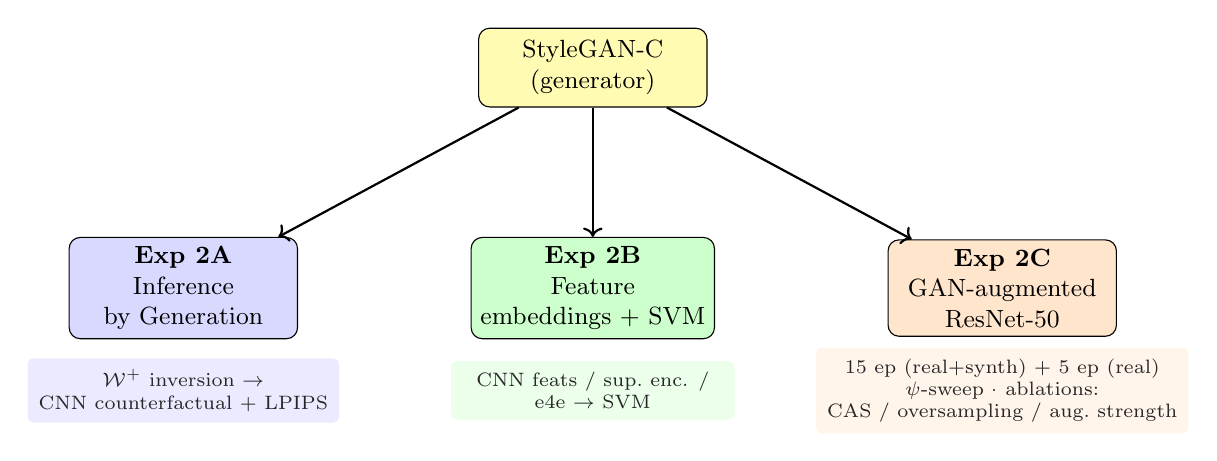
\begin{tikzpicture}[
    box/.style={draw,rounded corners,minimum width=2.9cm,
                minimum height=1cm,align=center,font=\small},
    arr/.style={->,thick},
    detail/.style={draw=none,fill=gray!8,rounded corners=2pt,
                   minimum width=3.6cm,inner sep=4pt,
                   font=\scriptsize,align=center,text=black!85},
    detailA/.style={detail,fill=blue!8},
    detailB/.style={detail,fill=green!8},
    detailC/.style={detail,fill=orange!8}
  ]
    \node[box,fill=yellow!30] (gan) at (0,0) {StyleGAN-C\\(generator)};

    \node[box,fill=blue!15]  (e1) at (-5.2,-2.8)
      {\textbf{Exp 2A}\\Inference\\by Generation};
    \node[box,fill=green!20] (e2) at (0,-2.8)
      {\textbf{Exp 2B}\\Feature\\embeddings + SVM};
    \node[box,fill=orange!20](e3) at (5.2,-2.8)
      {\textbf{Exp 2C}\\GAN-augmented\\ResNet-50};

    \node[detailA] at (-5.2,-4.1)
      {$\mathcal{W}^+$ inversion $\to$\\CNN counterfactual + LPIPS};
    \node[detailB] at (0,-4.1)
      {CNN feats / sup.\ enc. /\\e4e $\to$ SVM};
    \node[detailC] at (5.2,-4.1)
      {15 ep (real+synth) + 5 ep (real)\\$\psi$-sweep · ablations:\\CAS / oversampling / aug.\ strength};

    \draw[arr] (gan) -- (e1);
    \draw[arr] (gan) -- (e2);
    \draw[arr] (gan) -- (e3);
  \end{tikzpicture}
  \end{center}
\end{frame}

% ── NEW: HITL & XAI Module ───────────────────────────────────
\begin{frame}{Methodology (4/4): Experiment 3 · HITL \& XAI}
  \footnotesize
  \begin{columns}
    \begin{column}{0.5\textwidth}
      \textbf{HITL protocol:} 1 neuroradiologist, blinded, randomized order;
      expert not informed of class or real-vs-synthetic.

      \vspace{0.4em}
      \textbf{Two-form design:}
      \begin{itemize}\itemsep1pt
        \item \textbf{Form A} (no XAI): Real/Fake judgment, Confidence 1--5, Utility 1--5
        \item \textbf{Form B} (with Grad-CAM): same + heatmap rating
      \end{itemize}

      \vspace{0.4em}
      \textbf{Heatmap rating:} \emph{yes} (full / partial) · \emph{no}.
      Grad-CAM extracted from the \textbf{Exp 2C ResNet-50} ensemble; shown as
      paired images (with vs.\ without overlay).
    \end{column}
    \begin{column}{0.46\textwidth}
      \begin{block}{Sample composition (n=33)}
        \scriptsize
        \begin{tabular}{lccc|c}
          \toprule
          Subset & Glio & Men & Pit & Total \\
          \midrule
          Real        & 5 & 5 & 5 & 15 \\
          Synthetic   & 6 & 6 & 6 & 18 \\
          \midrule
          \textbf{Total} & \textbf{11} & \textbf{11} & \textbf{11} & \textbf{33} \\
          \bottomrule
        \end{tabular}
        \vspace{2pt}
        \scriptsize \textit{Pilot feasibility study; balanced per class.}
      \end{block}
      \vspace{0.4em}
      \begin{exampleblock}{Metrics collected}
        \scriptsize Diagnostic accuracy ·
        Confidence (1--5) · Utility (1--5) ·
        Heatmap rating (yes/partial/no).
      \end{exampleblock}
    \end{column}
  \end{columns}
\end{frame}

% ============================================================
%  SLIDES — RESULTS
% ============================================================
\section{Results}
\begin{frame}{Results (1/7): Generation Quality}
  \begin{columns}[T]
    \begin{column}{0.49\textwidth}
      {\setbeamercolor{block title}{bg=myblue!85, fg=white}%
       \setbeamercolor{block body}{bg=myblue!10, fg=black}%
      \begin{block}{FID · lower is better}
        \scriptsize
        Distributional similarity in Inception-v3 feature space.\\[3pt]
        \begin{tabular*}{\linewidth}{@{\extracolsep{\fill}}llcc}
          \toprule
          Method & Work & Dataset & FID \\
          \midrule
          DCGAN        & Ghassemi (2020) & Figshare   & n/a \\
          TumorGAN     & Li (2020)       & BraTS 2017 & 77.43 \\
          LR-cGAN      & Zhan (2021)     & BraTS 2015 & n/a \\
          MCFDiffusion & Zuo (2025)      & LGG        & 70.58 \\
          \midrule
          \textbf{StyleGAN-C} & \textbf{This thesis} & \textbf{Figshare} & \textbf{46.08} \\
          \bottomrule
        \end{tabular*}\\[2pt]
        \textit{Not directly comparable: different datasets/protocols.}
      \end{block}}
    \end{column}
    \begin{column}{0.49\textwidth}
      {\setbeamercolor{block title}{bg=mygreen!75, fg=white}%
       \setbeamercolor{block body}{bg=mygreen!10, fg=black}%
      \begin{block}{FID vs.\ truncation $\psi$ (reduced)}
        \begin{center}
        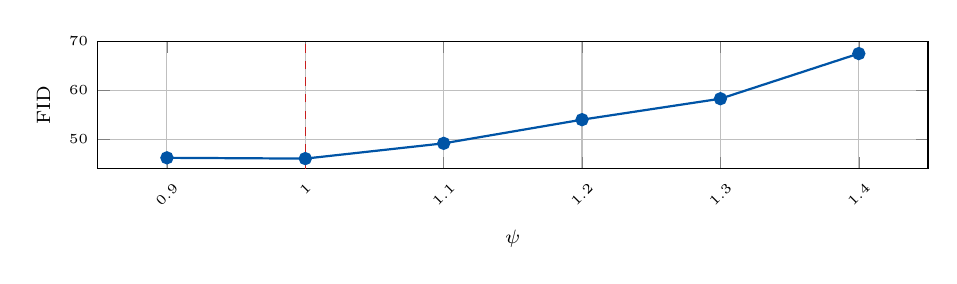
\begin{tikzpicture}
          \begin{axis}[
            xlabel={\scriptsize $\psi$},
            ylabel={\scriptsize FID},
            ymin=44, ymax=70,
            xtick={0.9,1.0,1.1,1.2,1.3,1.4},
            xticklabel style={font=\tiny,rotate=45},
            yticklabel style={font=\tiny},
            width=\linewidth, height=3.2cm,
            grid=major, mark size=2pt,
          ]
            \addplot[thick,myblue,mark=*] coordinates {
              (0.9,46.239)(1.0,46.08)
              (1.1,49.192)(1.2,54.024)(1.3,58.296)(1.4,67.509)
            };
            \draw[dashed,myred] (axis cs:1.0,44) -- (axis cs:1.0,70)
              node[above,font=\tiny] {$\psi^*=1.0$};
          \end{axis}
        \end{tikzpicture}
        \end{center}
      \end{block}}
    \end{column}
  \end{columns}

  \vspace{0.3em}
  \begin{center}
  \begin{minipage}{0.6\textwidth}
    {\setbeamercolor{block title}{bg=mygold!85, fg=white}%
     \setbeamercolor{block body}{bg=mygold!10, fg=black}%
    \begin{block}{\centering CAS · Classifier accuracy on synthetics\hfill}
      \scriptsize
      \begin{center}
      Classifier trained only on real data, evaluated on synthetic images.\\[2pt]
      \textbf{CAS = 92.3\%} \;($\psi{=}1.0$, $N{=}400$/class)
      \end{center}
    \end{block}}
  \end{minipage}
  \end{center}
\end{frame}

\begin{frame}{Results (2/7): Exp 2A · Inference by Generation}
  \footnotesize
  \begin{columns}[T]
    \begin{column}{0.48\textwidth}
      \begin{block}{\centering LPIPS \;($n=68$)\hfill}
        \scriptsize
        \begin{tabular*}{\linewidth}{@{\extracolsep{\fill}}lccc}
          \toprule
          Class & Precision & Recall & F1 \\
          \midrule
          Glioma     & 80.0\% & 82.8\% & 81.4\% \\
          Meningioma & 72.2\% & 61.9\% & 66.7\% \\
          Pituitary  & 75.0\% & 83.3\% & 78.9\% \\
          \midrule
          \multicolumn{4}{c}{\textbf{Overall accuracy: 76.5\%}} \\
          \bottomrule
        \end{tabular*}
      \end{block}
    \end{column}
    \begin{column}{0.48\textwidth}
      \begin{block}{\centering CNN \;($n=68$)\hfill}
        \scriptsize
        \begin{tabular*}{\linewidth}{@{\extracolsep{\fill}}lccc}
          \toprule
          Class & Precision & Recall & F1 \\
          \midrule
          Glioma     & 91.3\% & 72.4\% & 80.8\% \\
          Meningioma & 67.9\% & 90.5\% & 77.6\% \\
          Pituitary  & 100\%  & 94.4\% & 97.1\% \\
          \midrule
          \multicolumn{4}{c}{\textbf{Overall accuracy: 83.8\%}} \\
          \bottomrule
        \end{tabular*}
      \end{block}
    \end{column}
  \end{columns}

  \vspace{0.3em}
  \begin{columns}[T]
    \begin{column}{0.36\textwidth}
      \begin{exampleblock}{XAI by-product}
        \scriptsize \textbf{Counterfactual video}: 120-frame linear interpolation in $\mathcal{W}^+$.\\[3pt]
        \textit{``What would this meningioma look like if it were a pituitary?''}
      \end{exampleblock}
    \end{column}
    \begin{column}{0.61\textwidth}
      \begin{center}
        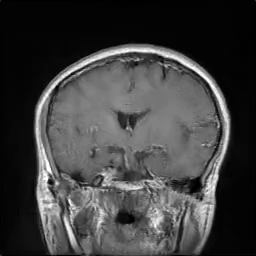
\includegraphics[width=0.18\linewidth]{img/cf_frames/cf_frame1.png}\hfill
        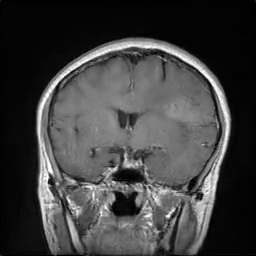
\includegraphics[width=0.18\linewidth]{img/cf_frames/cf_frame2.png}\hfill
        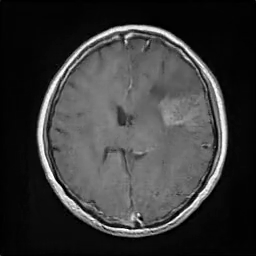
\includegraphics[width=0.18\linewidth]{img/cf_frames/cf_frame3.png}\hfill
        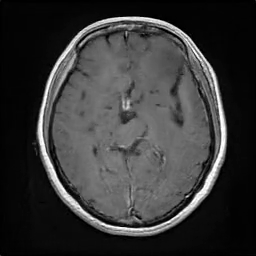
\includegraphics[width=0.18\linewidth]{img/cf_frames/cf_frame4.png}\hfill
        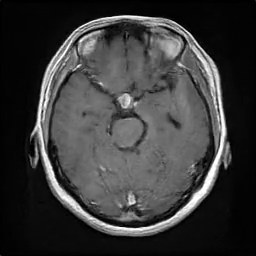
\includegraphics[width=0.18\linewidth]{img/cf_frames/cf_frame5.png}\\[2pt]
        {\tiny\itshape meningioma $\;\longrightarrow\;$ pituitary (5 frames)}
      \end{center}
    \end{column}
  \end{columns}
\end{frame}

\begin{frame}{Results (3/7): Exp 2B · Feature Embeddings + SVM}
  \begin{columns}
    \begin{column}{0.55\textwidth}
      \begin{center}
      \scriptsize
      \begin{tabular*}{0.95\linewidth}{@{\extracolsep{\fill}}lccc}
        \toprule
        Feature & Dim & Acc. & PCA \\
        \midrule
        e4e ($W^+$)          & 7{,}168 & 83.2\% & 53.8\% \\
        CNN ResNet-50        & 2{,}048 & 93.7\% & 64.7\% \\
        \textbf{Supervised}  & \textbf{512} & \textbf{94.7\%} & \textbf{99.4\%} \\
        \bottomrule
      \end{tabular*}
      \end{center}

      \vspace{0.4em}
      \begin{exampleblock}{\centering Best model · Supervised encoder + SVM\hfill}
        \begin{center}
        \scriptsize
        \begin{tabular*}{0.95\linewidth}{@{\extracolsep{\fill}}lccc}
          \toprule
          Class       & Precision & Recall & F1 \\
          \midrule
          Glioma      & 97.0\%    & 94.8\% & 95.9\% \\
          Meningioma  & 85.1\%    & 91.2\% & 88.1\% \\
          Pituitary   & 98.5\%    & 97.0\% & 97.8\% \\
          \midrule
          \multicolumn{4}{c}{\textbf{Overall accuracy: 94.7\%}} \\
          \bottomrule
        \end{tabular*}
        \end{center}
      \end{exampleblock}
    \end{column}
    \begin{column}{0.43\textwidth}
      \begin{block}{Reading}
        \footnotesize
        The \textbf{supervised encoder} collapses its representation toward
        the 2 discriminant axes needed for a 3-class problem
        (99.4\% variance in PC1+PC2).

        \vspace{0.4em}
        $\textbf{e4e}$ (designed for face inversion) gives weaker features
        even after fine-tuning on brain MRI; the $\mathcal{W}^+$ space
        optimizes for reconstruction, not class separation.

        \vspace{0.4em}
        \textbf{CNN features} sit in the middle: discriminatively trained,
        but the high-dim space (2{,}048) is less compact than the supervised
        encoder's 512-d embedding.
      \end{block}
    \end{column}
  \end{columns}
\end{frame}

\begin{frame}{Results (4/7): Exp 2C · GAN-augmented Classification}
  \begin{columns}
    \begin{column}{0.43\textwidth}
      \begin{block}{Reading}
        \footnotesize
        Best result is \textbf{GAN-aug $\psi{=}1.3$ ensemble (96.0\%)},
        narrowly above strong geometric augmentation (95.9\%).

        \vspace{0.4em}
        Per-class: \textbf{pituitary} is easiest (98.6\% F1),
        \textbf{meningioma} is hardest (91.5\% F1), consistent with its
        underrepresentation and visual variability.
      \end{block}
    \end{column}
    \begin{column}{0.55\textwidth}
      \begin{center}
      \scriptsize
      \begin{tabular*}{0.95\linewidth}{@{\extracolsep{\fill}}lcc}
        \toprule
        Configuration & F1 & Acc. \\
        \midrule
        Naive oversampling                      & 92.1\% & 93.4\% \\
        Real-only ensemble                      & 94.5\% & 95.3\% \\
        Strong geometric aug.                   & 95.2\% & 95.9\% \\
        \textbf{GAN-aug ($\psi{=}1.3$)}         & \textbf{95.4\%} & \textbf{96.0\%} \\
        \bottomrule
      \end{tabular*}
      \end{center}

      \vspace{0.4em}
      \begin{exampleblock}{\centering Best model · GAN-aug ($\psi=1.3$, reduced)\hfill}
        \begin{center}
        \scriptsize
        \begin{tabular*}{0.95\linewidth}{@{\extracolsep{\fill}}lccc}
          \toprule
          Class       & Precision & Recall & F1 \\
          \midrule
          Glioma      & 95.8\%    & 96.2\% & 96.0\% \\
          Meningioma  & 90.9\%    & 92.2\% & 91.5\% \\
          Pituitary   & 99.2\%    & 98.0\% & 98.6\% \\
          \midrule
          \multicolumn{4}{c}{\textbf{Overall accuracy: 96.0\%}} \\
          \bottomrule
        \end{tabular*}
        \end{center}
      \end{exampleblock}
    \end{column}
  \end{columns}
\end{frame}

\begin{frame}{Results (5/7): Leakage \& Statistical Tests}
  \begin{columns}[T]
    \begin{column}{0.6\textwidth}
      \textbf{Leakage configurations (5-fold ensemble):}\\[4pt]
      \scriptsize
      \begin{tabular*}{\linewidth}{@{\extracolsep{\fill}}lccc}
        \toprule
        Setup & Split leak & Generator leak & Accuracy \\
        \midrule
        \textcolor{mygreen}{\textbf{Clean baseline}}     & no  & no  & 95.2\% \\
        \textcolor{mygold}{Split-only leak}              & yes & no  & 97.9\% \\
        \textcolor{myred}{\textbf{Both leak}}            & yes & yes & \textbf{98.5\%} \\
        \bottomrule
      \end{tabular*}
      \vspace{0.4em}
      \normalsize
      \begin{itemize}\scriptsize
        \item Split leakage alone $\Rightarrow$ \textbf{+2.7\,pp} (95.2 $\to$ 97.9)
        \item Adding generator leakage on top $\Rightarrow$ \textbf{+3.3\,pp} total (98.5\%)
      \end{itemize}
      \vspace{0.2em}
      {\tiny\itshape Split leak = slice-level random train/test split (patients overlap);
      Generator leak = GAN trained on all images including test patients ($\psi=1.3$).}
    \end{column}
    \begin{column}{0.38\textwidth}
      \textbf{Statistical tests (reduced):}\\[4pt]
      \scriptsize
      \begin{tabular*}{\linewidth}{@{\extracolsep{\fill}}lc}
        \toprule
        Test & $p < 0.05$ \\
        \midrule
        McNemar: ens.\ vs.\ 1-run & \textcolor{mygreen}{$\checkmark$} \\
        McNemar: Real vs.\ GAN    & \textcolor{myred}{$\times$} \\
        NLL: Real vs.\ GAN        & \textcolor{mygreen}{$\checkmark$} \\
        \bottomrule
      \end{tabular*}
      \vspace{0.1em}
      {\tiny\itshape \textcolor{mygreen}{$\checkmark$} = significant ($p<0.05$),
      \textcolor{myred}{$\times$} = not.}
      \vspace{0.4em}
      \begin{block}{}
        \scriptsize
        \textbf{1.}\;Ensembling 5-fold models gives significantly better predictions than any single fold.\\[2pt]
        \textbf{2.}\;GAN augmentation does \emph{not} significantly change \textbf{which} samples are classified correctly.\\[2pt]
        \textbf{3.}\;GAN augmentation \emph{does} significantly improve \textbf{how confidently} correct predictions are made (lower NLL).
      \end{block}
    \end{column}
  \end{columns}
\end{frame}

\begin{frame}{Results (6/7): Augmentation Ablation Study}
  \begin{center}
  \begin{tabular}{lcccc}
    \toprule
    Configuration & Acc. & Precision & Recall & F1 \\
    \midrule
    Naive oversampling          & 93.4\% & 0.918 & 0.925 & 0.921 \\
    Weak geometric aug.         & 93.2\% & 0.915 & 0.921 & 0.918 \\
    Strong geometric aug.       & 95.9\% & 0.951 & 0.953 & 0.952 \\
    \midrule
    \textbf{GAN ($\psi=1.3$, ours)} & \textbf{96.0\%} & \textbf{0.953} & \textbf{0.954} & \textbf{0.954} \\
    \bottomrule
  \end{tabular}
  \end{center}
  \vspace{0.4em}
  \begin{itemize}\small
    \item Strong geometric augmentation alone is a competitive baseline (95.9\%)
    \item Naive oversampling does \emph{not} help: the model already memorizes minority classes
    \item GAN augmentation matches strong-aug accuracy and significantly improves \textbf{calibration} ($p < 0.05$)
  \end{itemize}
\end{frame}

\begin{frame}{Results (7/7): HITL \& Grad-CAM}
  \footnotesize
  \textbf{HITL protocol:} 1 neuroradiologist, 33 images, blinded reading.

  \vspace{0.2em}
  \begin{columns}[T]
    \begin{column}{0.34\textwidth}
      \begin{minipage}[t][2.9cm][t]{\linewidth}
      \textit{\scriptsize Real vs.\ synth.\ by class:}\\[3pt]
      \tiny
      \begin{tabular*}{\linewidth}{@{\extracolsep{\fill}}lcccc}
        \toprule
        Subset & $n$ & Acc & Conf & Util \\
        \midrule
        Real (all)              & 15 & \textbf{100\%} & 3.73 & 3.80 \\
        Synth.\ (all)           & 18 & \textbf{50\%}  & 2.22 & 2.11 \\
        \;glioma                & 6  & 50\%           & 1.67 & 1.67 \\
        \;meningioma            & 6  & \textcolor{myred}{17\%} & 1.67 & 1.33 \\
        \;pituitary             & 6  & 83\%           & 3.33 & 3.33 \\
        \bottomrule
      \end{tabular*}
      \end{minipage}

      \vspace{0.2em}
      \begin{center}
      \begin{minipage}{0.92\linewidth}
      {\setbeamercolor{block title}{bg=myblue!85, fg=white}%
       \setbeamercolor{block body}{bg=myblue!10, fg=black}%
      \begin{block}{}\tiny
        \begin{itemize}\itemsep1pt\setlength{\leftmargini}{1em}
          \item Real: 100\% acc, conf 3.73
          \item Synth: 50\% acc (expert often refused), conf 2.22
          \item \textbf{Pituitary} easiest (83\%, util 3.33)
          \item \textbf{Meningioma} hardest (17\%, util 1.33)
        \end{itemize}
      \end{block}}
      \end{minipage}
      \end{center}
    \end{column}
    \begin{column}{0.32\textwidth}
      \begin{minipage}[t][2.9cm][t]{\linewidth}
      \textit{\scriptsize By XAI pairing:}\\[3pt]
      \tiny
      \begin{tabular*}{\linewidth}{@{\extracolsep{\fill}}lcccc}
        \toprule
        Subset & $n$ & Acc & Conf & Util \\
        \midrule
        \textbf{XAI paired}     & 18 & 0.78 & 3.28 & 3.33 \\
        \;real                  & 9  & 1.00 & 3.56 & 3.67 \\
        \;synth.                & 9  & \textbf{0.56} & 3.00 & 3.00 \\
        \textbf{XAI not paired} & 15 & 0.67 & 2.47 & 2.33 \\
        \;real                  & 6  & 1.00 & 4.00 & 4.00 \\
        \;synth.                & 9  & \textbf{0.44} & 1.44 & 1.22 \\
        \bottomrule
      \end{tabular*}
      \end{minipage}

      \vspace{0.2em}
      \begin{center}
      \begin{minipage}{0.92\linewidth}
      {\setbeamercolor{block title example}{bg=mygreen!75, fg=white}%
       \setbeamercolor{block body example}{bg=mygreen!10, fg=black}%
      \begin{exampleblock}{}\tiny
        \begin{itemize}\itemsep1pt\setlength{\leftmargini}{1em}
          \item Synth.\ accuracy: 0.44 $\to$ 0.56
          \item \textbf{Synth.\ confidence: 1.44 $\to$ 3.00}
          \item Synth.\ utility: 1.22 $\to$ 3.00
          \item Real images unchanged (100\%)
        \end{itemize}
      \end{exampleblock}}
      \end{minipage}
      \end{center}
    \end{column}
    \begin{column}{0.32\textwidth}
      \begin{minipage}[t][2.9cm][t]{\linewidth}
      \textit{\scriptsize By heatmap quality:}\\[3pt]
      \tiny
      \begin{tabular*}{\linewidth}{@{\extracolsep{\fill}}lcccc}
        \toprule
        Heatmap & $n$ & Acc & Conf & Util \\
        \midrule
        \multicolumn{5}{l}{\textit{Real}} \\
        \;Correct      & 6 & 100\%          & 3.50 & 3.67 \\
        \;Rated ``no'' & 3 & 100\%          & 3.67 & 3.67 \\
        \midrule
        \multicolumn{5}{l}{\textit{Synthetic}} \\
        \;\textcolor{mygreen}{Correct}    & 3 & \textbf{100\%} & 4.33 & 4.33 \\
        \;\textcolor{myred}{Rated ``no''} & 6 & \textbf{33\%}  & 2.33 & 2.33 \\
        \bottomrule
      \end{tabular*}
      \end{minipage}

      \vspace{0.2em}
      \begin{center}
      \begin{minipage}{0.92\linewidth}
      {\setbeamercolor{block title alerted}{bg=mygold!85, fg=white}%
       \setbeamercolor{block body alerted}{bg=mygold!10, fg=black}%
      \begin{alertblock}{}\tiny
        \begin{itemize}\itemsep1pt\setlength{\leftmargini}{1em}
          \item Synth.\ correct heatmap: \textbf{100\%}, conf 4.33
          \item Synth.\ wrong heatmap: \textbf{33\%}, conf 2.33
          \item Real images: always 100\%
        \end{itemize}
      \end{alertblock}}
      \end{minipage}
      \end{center}
    \end{column}
  \end{columns}
\end{frame}

% ============================================================
%  SLIDES 16–17 — DISCUSSION
% ============================================================
\section{Discussion}
\begin{frame}{Discussion (1/2): Per-Experiment Findings}
  \scriptsize
  \begin{columns}[T]
    \begin{column}{0.49\textwidth}
      \begin{minipage}[t][0.82\textheight][s]{\linewidth}
      {\setbeamercolor{block title}{bg=myblue!85, fg=white}%
       \setbeamercolor{block body}{bg=myblue!10, fg=black}%
      \begin{block}{Exp 1: Image Generation}
        Synthetic images cannot fool an expert, but for classification tasks they perform well: \textbf{CAS 92.3\%}, \textbf{FID 46.08} (best on Figshare). Quality is class-dependent (pituitary $>$ glioma $>$ meningioma).
      \end{block}}

      \vfill
      {\setbeamercolor{block title}{bg=mygold!85, fg=white}%
       \setbeamercolor{block body}{bg=mygold!10, fg=black}%
      \begin{block}{Exp 2A: Inference by Generation}
        Only \textbf{83.8\%}; latent inversion (+5h) costly and far below CNN baseline. Tests an alternative paradigm (generation-based classification).
      \end{block}}

      \vfill
      {\setbeamercolor{block title}{bg=mypurple!85, fg=white}%
       \setbeamercolor{block body}{bg=mypurple!10, fg=black}%
      \begin{block}{Exp 2B: Encoder + SVM}
        Encoder + SVM is a viable form of classification: \textbf{94.7\%}. Competitive but still below GAN-augmented CNN.
      \end{block}}
      \end{minipage}
    \end{column}
    \begin{column}{0.49\textwidth}
      \begin{minipage}[t][0.82\textheight][s]{\linewidth}
      {\setbeamercolor{block title}{bg=mygreen!85, fg=white}%
       \setbeamercolor{block body}{bg=mygreen!10, fg=black}%
      \begin{block}{Exp 2C: GAN Augmentation}
        GAN-aug (\textbf{96.0\%}) $\approx$ strong-aug (95.9\%) on accuracy, but GAN delivers \textbf{better calibration}. Benefit is largest under data scarcity (reduced dataset).
      \end{block}}

      \vfill
      {\setbeamercolor{block title}{bg=myred!85, fg=white}%
       \setbeamercolor{block body}{bg=myred!10, fg=black}%
      \begin{block}{Exp 3: Pilot HITL + Grad-CAM}
        $\sim$50\% of synth slices diagnosable; Grad-CAM raises confidence
        \textbf{1.44 $\to$ 3.00} on synth, but only when the heatmap is accurate (wrong heatmaps drop accuracy to 33\%). A heatmap quality classifier is needed before clinical deployment.
      \end{block}}

      \vfill
      \phantom{X}
      \end{minipage}
    \end{column}
  \end{columns}
\end{frame}

\begin{frame}{Discussion (2/2): Leakage \& Clinical Implications}
  \scriptsize
  \begin{columns}[T]
    \begin{column}{0.62\textwidth}
      {\setbeamercolor{block title alerted}{bg=myred!85, fg=white}%
       \setbeamercolor{block body alerted}{bg=myred!10, fg=black}%
      \begin{alertblock}{Leakage impact on the literature}
        \begin{itemize}\itemsep1pt
          \item $\sim$3 pp inflation quantified empirically
          \item Papers reporting $\sim$98\% (no patient control) correspond to $\sim$95\% under fair evaluation
          \item Direct leaderboard comparisons on Figshare are potentially misleading
          \item \textbf{Proposal:} patient-level split must become a mandatory evaluation criterion
        \end{itemize}
      \end{alertblock}}

      \vspace{0.4em}
      {\setbeamercolor{block title}{bg=mygold!85, fg=white}%
       \setbeamercolor{block body}{bg=mygold!10, fg=black}%
      \begin{block}{Acknowledged Limitations}
        \begin{itemize}\itemsep1pt
          \item Single dataset (Figshare, one institution)
          \item Pilot HITL: only 1 neuroradiologist (small expert sample)
          \item High computational cost (synthetic generation + retraining)
          \item Partial generative validity ($\sim$50\% synth diagnostic; class-dependent)
        \end{itemize}
      \end{block}}
    \end{column}
    \begin{column}{0.36\textwidth}
      {\setbeamercolor{block title}{bg=myblue!85, fg=white}%
       \setbeamercolor{block body}{bg=myblue!10, fg=black}%
      \begin{block}{Why this matters clinically}
        \begin{itemize}\itemsep1pt
          \item Generator $\to$ class balancing, privacy-safe data sharing, training simulators
          \item Pilot HITL bridges \textbf{medicine $\leftrightarrow$ engineering}: reusable protocol, scalable to multi-reader
          \item XAI: Grad-CAM + counterfactual $\to$ interpretable explanations clinicians can interrogate $\to$ more trustworthy model
          \item Telemedicine: AI assistance in regions with limited specialists
          \item Methodology extends to other tumors (lung, breast, prostate)
        \end{itemize}
      \end{block}}
    \end{column}
  \end{columns}
\end{frame}

% ============================================================
%  SLIDES 18–19 — CONCLUSIONS
% ============================================================
\section{Conclusions}
\begin{frame}{Conclusions (1/2): Findings \& Hypotheses}
  \footnotesize
  \textbf{Findings $\to$ research-question verdict:}
  \footnotesize
  \begin{enumerate}\itemsep2pt
    \item \textbf{Generation (RQ1):} FID 46.08, CAS 92.3\%.
          \textit{``Generated images are highly useful for the machine and classifier, but for the expert only some images are useful.''}
    \item \textbf{Classification (RQ2):} GAN aug improves calibration; 96\% vs 83.8\% (inversion).
          \textit{``StyleGAN-C performs better as an image generation model complementing classification models than for classification via inversion.''}
    \item \textbf{XAI (RQ3):} Grad-CAM raises synth confidence $1.44 \to 3.00$.
          \textit{``Grad-CAM is particularly useful for synthetic images.''}
    \item \textbf{Bonus -- Leakage:} $95.2\% \to 97.9\% \to 98.5\%$ ($\approx$3 pp inflation).
          \textit{Patient-level split must be a mandatory evaluation criterion.}
  \end{enumerate}

  \vspace{0.5em}
  \begin{center}
    \textbf{\footnotesize Hypotheses:}\\[3pt]
    \tiny
    \renewcommand{\arraystretch}{1.15}
    \begin{tabular}{@{}llp{4.5cm}@{}}
      \toprule
      H & Status & Evidence \\
      \midrule
      H1 (plausible MRI)   & \textcolor{mygold}{partial}   & 50\% diag.; CAS 92.3\% \\
      H2A (latent inv.)    & \textcolor{mygreen}{\checkmark} & 83.8\% accuracy (Exp 2A) \\
      H2B (calibration)    & \textcolor{mygreen}{\checkmark} & Better calibration \\
      H3 (XAI utility)     & \textcolor{mygold}{partial}   & Synth conf.\ 1.44 $\to$ 3.00 \\
      \bottomrule
    \end{tabular}
  \end{center}
\end{frame}

\begin{frame}{Conclusions (2/2): Contributions \& Best Result}
  \footnotesize
  {\setbeamercolor{block title}{bg=myblue!85, fg=white}%
   \setbeamercolor{block body}{bg=myblue!10, fg=black}%
  \begin{block}{Contributions}
    \begin{enumerate}\itemsep2pt
      \item Class-conditional StyleGAN-C generator (FID best on Figshare)
      \item CNN classifier with strict leakage control (96\% accuracy)
      \item First pilot HITL protocol for synthetic + Grad-CAM review; CAS-based evaluation of synthetic quality
    \end{enumerate}
  \end{block}}

  \vspace{0.6em}
  \begin{block}{Best result of this work}
    \begin{center}
    \Large\textbf{96.0\% accuracy (patient-level)}\\[4pt]
    \normalsize
    5-fold ResNet-50 ensemble with GAN augmentation ($\psi=1.3$),\\
    reduced dataset, strict patient-level leakage control.\\[4pt]
    Precision (macro): 95.3\% $\cdot$ Recall (macro): 95.4\% $\cdot$ F1 (macro): 95.4\%
    \end{center}
  \end{block}
\end{frame}

% ============================================================
%  SLIDE 20 — FUTURE WORK
% ============================================================
\section{Future Work}
\begin{frame}{Future Work}
  \footnotesize
  \begin{columns}[T]
    \begin{column}{0.5\textwidth}
      \textbf{Methodological:}
      \begin{itemize}\itemsep2pt
        \item External validation: multi-center, multi-scanner cohorts (1.5T/3T)
        \item 3D volumetric / tri-planar inputs (axial $+$ sagittal $+$ coronal)
        \item Data curation + synthetic filtering
        \item Disentangled / controllable latent spaces (editable tumor morphology)
        \item Multimodal fusion: clinical metadata (age, sex), LLMs (GPT-4o, Gemini)
      \end{itemize}
    \end{column}
    \begin{column}{0.48\textwidth}
      \textbf{Clinical:}
      \begin{itemize}\itemsep2pt
        \item Multi-reader HITL study ($\geq$10 neuroradiologists)
        \item Pre-registered protocol with power analysis
        \item Grad-CAM heatmap quality classifier (XAI safety filter)
        \item Clinical decision support system (DSS) integration
      \end{itemize}
    \end{column}
  \end{columns}
\end{frame}

% ── FINAL SLIDE ───────────────────────────────────────────────
\customtitlepage

% ── BACKUP SLIDES ─────────────────────────────────────────────
\appendix

\begin{frame}{[Appendix] StyleGAN-C Generation Pipeline}
  \begin{center}
    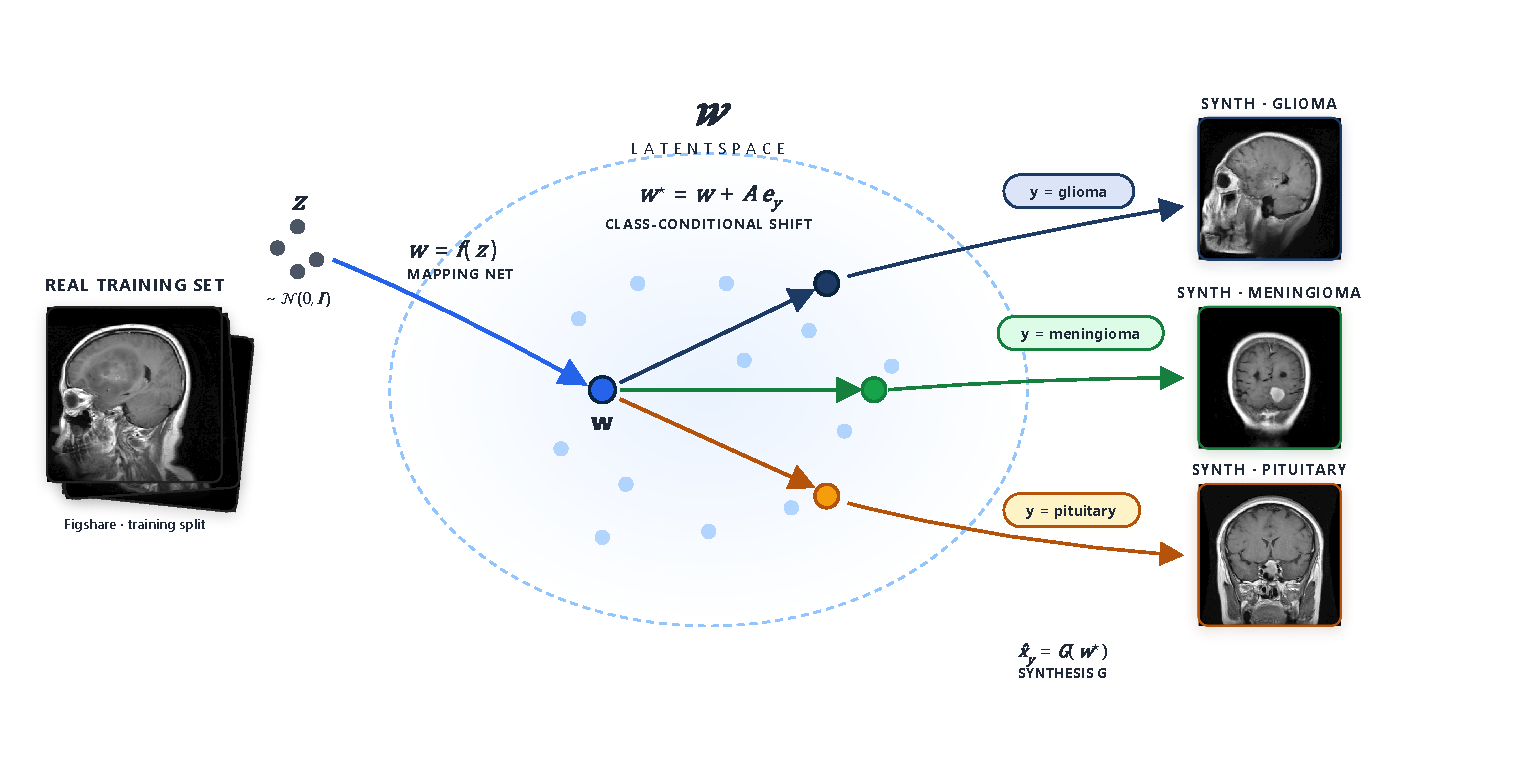
\includegraphics[width=0.98\textwidth]{img/diagram/diagram.pdf}
  \end{center}
  \vspace{-0.4em}
  {\scriptsize One $z$, three class shifts $A\,e_y$ $\to$ three class-specific images $\hat x_y$.}
\end{frame}

\begin{frame}{[Appendix] Per-class NLL · Where Does the Gain Come From?}
  \begin{center}
  \scriptsize
  \begin{tabular}{lcccccc}
    \toprule
    & \multicolumn{3}{c}{\textbf{Reduced dataset}} & \multicolumn{3}{c}{\textbf{Complete dataset}} \\
    \cmidrule(lr){2-4}\cmidrule(lr){5-7}
    Class & Real & Synth. & $p$-value & Real & Synth. & $p$-value \\
    \midrule
    Global      & 0.105 & \textbf{0.091} & \textbf{0.0065} & 0.122 & 0.128 & 0.508 \\
    Glioma      & 0.124 & \textbf{0.086} & $<10^{-5}$       & 0.086 & 0.095 & 0.310 \\
    Meningioma  & 0.160 & 0.175 & 0.456                    & 0.253 & 0.307 & 0.137 \\
    Pituitary   & 0.051 & 0.049 & 0.713                    & 0.086 & \textbf{0.054} & $<10^{-5}$ \\
    \bottomrule
  \end{tabular}
  \end{center}
  \vspace{0.4em}
  {\footnotesize Reduced-dataset gain is driven by \textbf{glioma}; complete-dataset gain by \textbf{pituitary}; meningioma never reaches significance.}
\end{frame}

\begin{frame}{[Appendix] Per-class Generation Quality}
  \begin{columns}
    \begin{column}{0.55\textwidth}
      \textbf{Reconstruction metrics (paired):}\\
      \scriptsize
      \begin{tabular}{lcccc}
        \toprule
        Class & PSNR (dB) & SSIM & LPIPS & FID \\
        \midrule
        Glioma     & $15.46\pm1.86$ & $0.543$ & $0.211$ & 123.9 \\
        Meningioma & $13.91\pm1.64$ & $0.474$ & $0.280$ & 142.1 \\
        Pituitary  & $13.30\pm1.63$ & $0.377$ & $0.264$ & 168.5 \\
        \midrule
        Overall    & $14.43\pm1.98$ & $0.478$ & $0.245$ & --- \\
        \bottomrule
      \end{tabular}
      \normalsize
    \end{column}
    \begin{column}{0.42\textwidth}
      \begin{block}{Reading}
        Glioma reconstructs best
        (highest PSNR/SSIM, lowest LPIPS).\\[4pt]
        Pituitary worst on PSNR/SSIM/FID
        (small sellar region).\\[4pt]
        Meningioma worst on LPIPS
        (perceptually most different).
      \end{block}
    \end{column}
  \end{columns}
\end{frame}

\begin{frame}{[Backup] Full Ablation Study}
  \begin{center}
  \begin{tabular}{lccc}
    \toprule
    Configuration & Acc. & NLL & $p$ (NLL) \\
    \midrule
    No augmentation (baseline) & 94.8\% & 0.121 & --- \\
    Naive oversampling          & 93.4\% & 0.118 & --- \\
    Weak geometric aug.         & 93.2\% & 0.115 & --- \\
    Strong geometric aug.       & 95.9\% & 0.098 & --- \\
    \textbf{GAN ($\psi=1.3$)}  & \textbf{96.0\%} & \textbf{0.091} & \textbf{0.0065} \\
    \bottomrule
  \end{tabular}
  \end{center}
\end{frame}

\begin{frame}{[Backup] Encoder PCA Geometry}
  \begin{center}
  \begin{tabular}{lcccc}
    \toprule
    Encoder & Dim & PC1 & PC2 & Total (2 PCs) \\
    \midrule
    e4e ($W^+$)          & 7{,}168 & --- & --- & 66\% (3 PCs) \\
    CNN (ResNet-50)       & 2{,}048 & --- & --- & 72\% (3 PCs) \\
    \textbf{Supervised}  & \textbf{512} & \textbf{58.9\%} & \textbf{40.7\%} & \textbf{99.7\%} \\
    \bottomrule
  \end{tabular}
  \end{center}
  \vspace{0.3em}
  The supervised encoder collapses its representation toward the 2 discriminant
  dimensions required for 3-class separation.
\end{frame}

% ============================================================
%  APPENDIX — IMAGES
% ============================================================

\newcommand{\gradcam}{img/gradcam}
\newcommand{\realfake}{img/realfake}
\newcommand{\proj}{img/projections}
\newcommand{\inttest}{img/inttest}
\newcommand{\cnnfold}{img/cnnfold}

% ── GROUP 1: REAL vs. SYNTHETIC ───────────────────────────────

\begin{frame}{[Appendix] Real vs.\ Synthetic — Glioma}
  \begin{columns}
    \begin{column}{0.5\textwidth}
      \centering\textbf{Real}\\[4pt]
      
\includegraphics[width=0.47\textwidth]{\realfake/real/glioma/88670_glioma_0012.png}\hfill
      
\includegraphics[width=0.47\textwidth]{\realfake/real/glioma/MR024780E_glioma_0006.png}\\[4pt]
      
\includegraphics[width=0.47\textwidth]{\realfake/real/glioma/MR026175E_glioma_0008.png}\hfill
      
\includegraphics[width=0.47\textwidth]{\realfake/real/glioma/MR039473B_glioma_0018.png}
    \end{column}
    \begin{column}{0.5\textwidth}
      \centering\textbf{Synthetic (StyleGAN-C)}\\[4pt]
      
\includegraphics[width=0.47\textwidth]{\realfake/fake/glioma/seed4506358.png}\hfill
      
\includegraphics[width=0.47\textwidth]{\realfake/fake/glioma/seed4603295.png}\\[4pt]
      
\includegraphics[width=0.47\textwidth]{\realfake/fake/glioma/seed4872550.png}\hfill
      
\includegraphics[width=0.47\textwidth]{\realfake/fake/glioma/seed5426986.png}
    \end{column}
  \end{columns}
\end{frame}

\begin{frame}{[Appendix] Real vs.\ Synthetic — Meningioma}
  \begin{columns}
    \begin{column}{0.5\textwidth}
      \centering\textbf{Real}\\[4pt]
      
\includegraphics[width=0.47\textwidth]{\realfake/real/meningioma/102446_meningioma_0002.png}\hfill
      
\includegraphics[width=0.47\textwidth]{\realfake/real/meningioma/102675_meningioma_0005.png}\\[4pt]
      
\includegraphics[width=0.47\textwidth]{\realfake/real/meningioma/104695_meningioma_0003.png}\hfill
      
\includegraphics[width=0.47\textwidth]{\realfake/real/meningioma/106720_meningioma_0014.png}
    \end{column}
    \begin{column}{0.5\textwidth}
      \centering\textbf{Synthetic (StyleGAN-C)}\\[4pt]
      
\includegraphics[width=0.47\textwidth]{\realfake/fake/meningioma/seed1791154.png}\hfill
      
\includegraphics[width=0.47\textwidth]{\realfake/fake/meningioma/seed33912.png}\\[4pt]
      
\includegraphics[width=0.47\textwidth]{\realfake/fake/meningioma/seed4803649.png}\hfill
      
\includegraphics[width=0.47\textwidth]{\realfake/fake/meningioma/seed5885214.png}
    \end{column}
  \end{columns}
\end{frame}

\begin{frame}{[Appendix] Real vs.\ Synthetic — Pituitary}
  \begin{columns}
    \begin{column}{0.5\textwidth}
      \centering\textbf{Real}\\[4pt]
      
\includegraphics[width=0.47\textwidth]{\realfake/real/pituitary/101305_pituitary_0008.png}\hfill
      
\includegraphics[width=0.47\textwidth]{\realfake/real/pituitary/103582_pituitary_0016.png}\\[4pt]
      
\includegraphics[width=0.47\textwidth]{\realfake/real/pituitary/107495_pituitary_0010.png}\hfill
      
\includegraphics[width=0.47\textwidth]{\realfake/real/pituitary/111125_pituitary_0011.png}
    \end{column}
    \begin{column}{0.5\textwidth}
      \centering\textbf{Synthetic (StyleGAN-C)}\\[4pt]
      
\includegraphics[width=0.47\textwidth]{\realfake/fake/pituitary/seed3264818.png}\hfill
      
\includegraphics[width=0.47\textwidth]{\realfake/fake/pituitary/seed6093501.png}\\[4pt]
      
\includegraphics[width=0.47\textwidth]{\realfake/fake/pituitary/seed6918384.png}\hfill
      
\includegraphics[width=0.47\textwidth]{\realfake/fake/pituitary/seed9138200.png}
    \end{column}
  \end{columns}
\end{frame}

% ── GROUP 2: GRAD-CAM OVERLAYS ────────────────────────────────

\begin{frame}{[Appendix] Grad-CAM — Glioma}
  \centering
  \begin{tabular}{cc}
    \textbf{Real (correctly classified)} &
    \textbf{Synthetic (correctly classified)} \\[4pt]
    
\includegraphics[width=0.42\textwidth]
      {\gradcam/glioma/glioma_true__glioma_pred__112027_glioma_0002.png} &
    
\includegraphics[width=0.42\textwidth]
      {\gradcam/glioma/glioma_true__glioma_pred__seed1172340.png} \\[6pt]
    
\includegraphics[width=0.42\textwidth]
      {\gradcam/glioma/glioma_true__glioma_pred__97609_glioma_0002.png} &
    
\includegraphics[width=0.42\textwidth]
      {\gradcam/glioma/glioma_true__glioma_pred__MR024780E_glioma_0006.png} \\
  \end{tabular}
  \vspace{2pt}
  \footnotesize Red zones = highest activation for the glioma class
\end{frame}

\begin{frame}{[Appendix] Grad-CAM — Meningioma}
  \centering
  \begin{tabular}{cc}
    \textbf{Real (correctly classified)} &
    \textbf{Synthetic (correctly classified)} \\[4pt]
    
\includegraphics[width=0.42\textwidth]
      {\gradcam/meningioma/meningioma_true__meningioma_pred__102960_meningioma_0002.png} &
    
\includegraphics[width=0.42\textwidth]
      {\gradcam/meningioma/meningioma_true__meningioma_pred__seed110646.png} \\[6pt]
    
\includegraphics[width=0.42\textwidth]
      {\gradcam/meningioma/meningioma_true__meningioma_pred__109411_meningioma_0003.png} &
    
\includegraphics[width=0.42\textwidth]
      {\gradcam/meningioma/meningioma_true__meningioma_pred__113614_meningioma_0001.png} \\
  \end{tabular}
  \vspace{2pt}
  \footnotesize Red zones = highest activation for the meningioma class
\end{frame}

\begin{frame}{[Appendix] Grad-CAM — Pituitary}
  \centering
  \begin{tabular}{cc}
    \textbf{Real (correctly classified)} &
    \textbf{Synthetic (correctly classified)} \\[4pt]
    
\includegraphics[width=0.42\textwidth]
      {\gradcam/pituitary/pituitary_true__pituitary_pred__101145_pituitary_0002.png} &
    
\includegraphics[width=0.42\textwidth]
      {\gradcam/pituitary/pituitary_true__pituitary_pred__seed2118118.png} \\[6pt]
    
\includegraphics[width=0.42\textwidth]
      {\gradcam/pituitary/pituitary_true__pituitary_pred__105475_pituitary_0004.png} &
    
\includegraphics[width=0.42\textwidth]
      {\gradcam/pituitary/pituitary_true__pituitary_pred__111125_pituitary_0011.png} \\
  \end{tabular}
  \vspace{2pt}
  \footnotesize Red zones = highest activation for the pituitary class
\end{frame}

% ── GROUP 3: LATENT PROJECTIONS ───────────────────────────────

\begin{frame}{[Appendix] $W^+$ Latent Inversion — Glioma}
  \centering
  \small Real image (left) $\to$ reconstruction from $W^+$ space (right)\\[6pt]
  \begin{tabular}{cccc}
    \textbf{Original} & \textbf{Reconstructed} &
    \textbf{Original} & \textbf{Reconstructed} \\[2pt]
    
\includegraphics[width=0.20\textwidth]
      {\proj/glioma/MR024780G_glioma_0004/target.png} &
    
\includegraphics[width=0.20\textwidth]
      {\proj/glioma/MR024780G_glioma_0004/proj.png} &
    
\includegraphics[width=0.20\textwidth]
      {\proj/glioma/MR024780G_glioma_0005/target.png} &
    
\includegraphics[width=0.20\textwidth]
      {\proj/glioma/MR024780G_glioma_0005/proj.png} \\[6pt]
    
\includegraphics[width=0.20\textwidth]
      {\proj/glioma/MR036496B_glioma_0014/target.png} &
    
\includegraphics[width=0.20\textwidth]
      {\proj/glioma/MR036496B_glioma_0014/proj.png} &
    
\includegraphics[width=0.20\textwidth]
      {\proj/glioma/MR048297_glioma_0007/target.png} &
    
\includegraphics[width=0.20\textwidth]
      {\proj/glioma/MR048297_glioma_0007/proj.png} \\
  \end{tabular}
\end{frame}

\begin{frame}{[Appendix] $W^+$ Latent Inversion — Meningioma \& Pituitary}
  \small Real image (left) $\to$ reconstruction from $W^+$ space (right)\\[4pt]
  \begin{columns}
    \begin{column}{0.48\textwidth}
      \centering\textbf{Meningioma}\\[4pt]
      \begin{tabular}{cc}
        \textbf{Original} & \textbf{Reconstructed} \\[2pt]
        
\includegraphics[width=0.44\textwidth]
          {\proj/meningioma/101082_meningioma_0001/target.png} &
        
\includegraphics[width=0.44\textwidth]
          {\proj/meningioma/101082_meningioma_0001/proj.png} \\
      \end{tabular}
    \end{column}
    \begin{column}{0.48\textwidth}
      \centering\textbf{Pituitary}\\[4pt]
      \begin{tabular}{cc}
        \textbf{Original} & \textbf{Reconstructed} \\[2pt]
        
\includegraphics[width=0.44\textwidth]
          {\proj/pituitary/101029_pituitary_0003/target.png} &
        
\includegraphics[width=0.44\textwidth]
          {\proj/pituitary/101029_pituitary_0003/proj.png} \\
      \end{tabular}
    \end{column}
  \end{columns}
  \vspace{0.3em}
  \footnotesize High reconstruction quality validates that $W^+$ space captures
  the diagnostically relevant information from real images.
\end{frame}

% ── GROUP 4: PERFORMANCE CURVES ───────────────────────────────

\begin{frame}{[Appendix] Accuracy vs.\ Number of Synthetic Images}
  \centering
  
\includegraphics[width=0.82\textwidth]{\inttest/inttest_accuracy_vs_nsyn.png}
  \vspace{4pt}
  \footnotesize Classifier accuracy trained with varying numbers of synthetic images
  per class (Integration Test).
\end{frame}

\begin{frame}{[Appendix] F1 Macro vs.\ Number of Synthetic Images}
  \centering
  
\includegraphics[width=0.82\textwidth]{\inttest/inttest_f1_macro_vs_nsyn.png}
  \vspace{4pt}
  \footnotesize Mean macro F1 per fold. The plateau justifies using $N=400$
  synthetic images per class as the optimal operating point.
\end{frame}

\begin{frame}{[Appendix] Precision \& Recall vs.\ Number of Synthetic Images}
  \begin{columns}
    \begin{column}{0.5\textwidth}
      \centering
      
\includegraphics[width=\textwidth]{\inttest/inttest_precision_macro_vs_nsyn.png}\\
      \footnotesize Macro Precision
    \end{column}
    \begin{column}{0.5\textwidth}
      \centering
      
\includegraphics[width=\textwidth]{\inttest/inttest_recall_macro_vs_nsyn.png}\\
      \footnotesize Macro Recall
    \end{column}
  \end{columns}
\end{frame}

\begin{frame}{[Appendix] Weighted F1, Precision \& Recall}
  \begin{columns}
    \begin{column}{0.33\textwidth}
      \centering
      
\includegraphics[width=\textwidth]{\inttest/inttest_f1_weighted_vs_nsyn.png}\\
      \footnotesize Weighted F1
    \end{column}
    \begin{column}{0.33\textwidth}
      \centering
      
\includegraphics[width=\textwidth]{\inttest/inttest_precision_weighted_vs_nsyn.png}\\
      \footnotesize Weighted Precision
    \end{column}
    \begin{column}{0.33\textwidth}
      \centering
      
\includegraphics[width=\textwidth]{\inttest/inttest_recall_weighted_vs_nsyn.png}\\
      \footnotesize Weighted Recall
    \end{column}
  \end{columns}
\end{frame}

\begin{frame}{[Appendix] Consolidated Plot — Macro F1}
  \centering
  
\includegraphics[width=0.82\textwidth]{\cnnfold/consolidated_plot_macroF1.png}
  \vspace{4pt}
  \footnotesize Consolidated comparison of all augmentation configurations
  in terms of macro F1 score.
\end{frame}

\end{document}
